
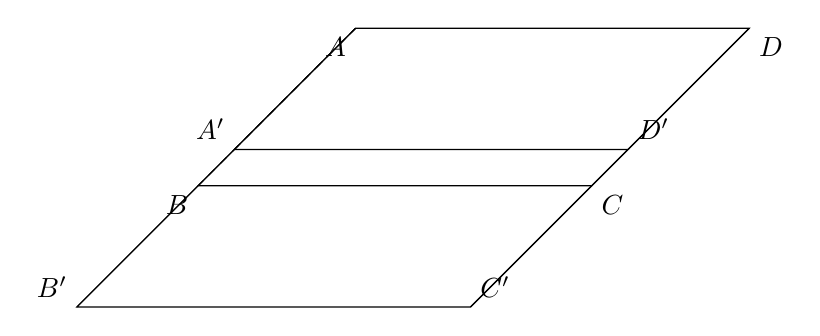
\begin{tikzpicture}
% Define coordinates
\coordinate (A) at (0,0,0);
\coordinate (B) at (-2,-2,0);
\coordinate (C) at (3,-2,0);
\coordinate (D) at (5,0,0);
\coordinate (A') at (0,0,4);
\coordinate (B') at (-2,-2,4);
\coordinate (C') at (3,-2,4);
\coordinate (D') at (5,0,4);

% Draw the front and top faces
\draw (A) -- (B) -- (C) -- (D) -- cycle; % Bottom face (solid lines)
\draw (A') -- (B') -- (C') -- (D') -- cycle; % Top face (solid lines)
\draw (A) -- (A'); % Vertical edge (solid)
\draw (B) -- (B'); % Vertical edge (solid)
\draw (C) -- (C'); % Vertical edge (solid)
\draw (D) -- (D'); % Vertical edge (solid)

% Draw hidden lines
\draw[dashed] (A) -- (D);
\draw[dashed] (A) -- (B);
\draw[dashed] (A') -- (A);

% Add labels
\node[below left] at (A) {$A$};
\node[below left] at (B) {$B$};
\node[below right] at (C) {$C$};
\node[below right] at (D) {$D$};
\node[above left] at (A') {$A'$};
\node[above left] at (B') {$B'$};
\node[above right] at (C') {$C'$};
\node[above right] at (D') {$D'$};

\end{tikzpicture}
